\documentclass[a4paper,
               %boxit,
               %titlepage,   % separate title page
               %refpage      % separate references
              ]{jacow}

\makeatletter%                           % test for XeTeX where the sequence is by default eps-> pdf, jpg, png, pdf, ...
\ifboolexpr{bool{xetex}}                 % and the JACoW template provides JACpic2v3.eps and JACpic2v3.jpg which might generates errors
 {\renewcommand{\Gin@extensions}{.pdf,%
                    .png,.jpg,.bmp,.pict,.tif,.psd,.mac,.sga,.tga,.gif,%
                    .eps,.ps,%
                    }}{}
\makeatother

\ifboolexpr{bool{xetex} or bool{luatex}} % test for XeTeX/LuaTeX
 {}                                      % input encoding is utf8 by default
 {\usepackage[utf8]{inputenc}}           % switch to utf8

\usepackage[USenglish]{babel}
\usepackage{balance}


\ifboolexpr{bool{jacowbiblatex}}%        % if BibLaTeX is used
 {%
  \addbibresource{jacow-test.bib}
  \addbibresource{biblatex-examples.bib}
 }{}

\newcommand\SEC[1]{\textbf{\uppercase{#1}}}

%%
%%   Lengths for the spaces in the title
%%   \setlength\titleblockstartskip{..}  %before title, default 3pt
%%   \setlength\titleblockmiddleskip{..} %between title + author, default 1em
%%   \setlength\titleblockendskip{..}    %afterauthor, default 1em

%\copyrightspace %default 1cm. arbitrary size with e.g. \copyrightspace[2cm]

% testing to fill the copyright space
%\usepackage{eso-pic}
%\AddToShipoutPictureFG*{\AtTextLowerLeft{\textcolor{red}{COPYRIGHTSPACE}}}

\begin{document}

\title{Integration of the Diamond Transverse Multibunch Feedback System at Alba}

\author{A. Olmos, U. Iriso, J. Moldes, F. P\'erez -- ALBA-CELLS, Cerdanyola (Spain) \\
M. Abbott, G. Rehm, I. Uzun -- Diamond Light Source, Oxfordshire (UK) }

\maketitle

%
\begin{abstract}
A Transverse Multi-Bunch Feedback system (TMBF) has been commissioned at the ALBA storage ring for stabilization of the beam instabilities. The system is based on the Libera Bunch-By-Bunch electronics, controlled using a specific software developed at Diamond Light Source. This system refurbishes the existing FPGA code to include several features for machine studies, like fast and precise tune measurements using a Phase Locked Loop, sequences of grow-damp experiments that allow measuring damping rates on a mode-by-mode basis, and precise bunch cleaning. We describe the TMBF system and the integration of the control software into the ALBA machine. We show examples of beam stabilization and machine studies using this system.

\end{abstract}


\section{Introduction}

Transverse betatron oscillations associated with coupled-bunch instabilities limit the machine performance in current synchrotron light sources. 
The TMBF system is designed to cure these instabilities by using an active feedback system based on sensors capable of detecting the beam motion, fast FPGA processors to calculate the motion correction, and actuators that apply the correction to the beam.

At ALBA, we have commissioned a TMBF system based on the Libera Bunch-By-Bunch electronics~\cite{iTech} provided by Instrumentation Technologies (ITech), controlled using the firmware and software developed at Diamond Light Source  (DLS)~\cite{DLS:IBIC15}. 
Since 2007, DLS has been developing functionality beyond the pure feedback action, and ALBA decided to profit from this experience. 

This paper describes the ALBA TMBF system, the integration of the control system from DLS to ALBA, and the performance and first results with it. 

\section{System Overview}

The block diagram of the ALBA TMBF is shown in Fig.~\ref{layout}. The signal coming from the BPM buttons is sent to the in-house Hybrid combiner designed to work around 1.5~GHz (3rd harmonic of the RF frequency) to maximize the transfer function. The Hybrid combines the four BPM signals to obtain the Horizontal, Vertical and Longitudinal (not used for the time being) components. Following to the Hybrid module, the RF FrontEnd, also by ITech, performs an amplitude and phase demodulation of the wideband components to the required working frequency of the following electronics. 

The Libera Bunch-by-Bunch unit is in charge of the detection of beam instabilities and the calculation of the corresponding correcting action (kick). Correct synchronization with bunches is accomplished by proper locking to 500~MHz RF clock, usage of timing signals from ALBA timing Event Receivers (EVR) and phase matching of all critical cables down to the picosecond range. Following to the Libera electronics, 180$^\circ$ splitters provide the drive for the 100~W / 50~dB / 250~MHz amplifiers by IFI. Signals from the amplifiers are sent through phase-matched cables to the feedback kickers (FFK) to act on the corresponding bunches. Forward signals out of the kickers are sent out of the tunnel for diagnostics purposes.

We have faced a problem on the amplifiers' phase response. While their 50~dB gain stays quite flat up to their higher working frequency (250~MHz), the amplifiers phase response starts degrading around 200~MHz, as it is shown in Fig.~\ref{AMPLI:GAIN} and Fig.~\ref{AMPLI:PHASE}. The effect of such amplifier imperfection is that when the system attempts to act on a particular bunch (while running the feedback, doing bunch cleaning etc.), it can happen that it also affects the neighbor bunches. In the future, we plan to change our amplifiers.


\begin{figure}[hbt!]
   \centering
   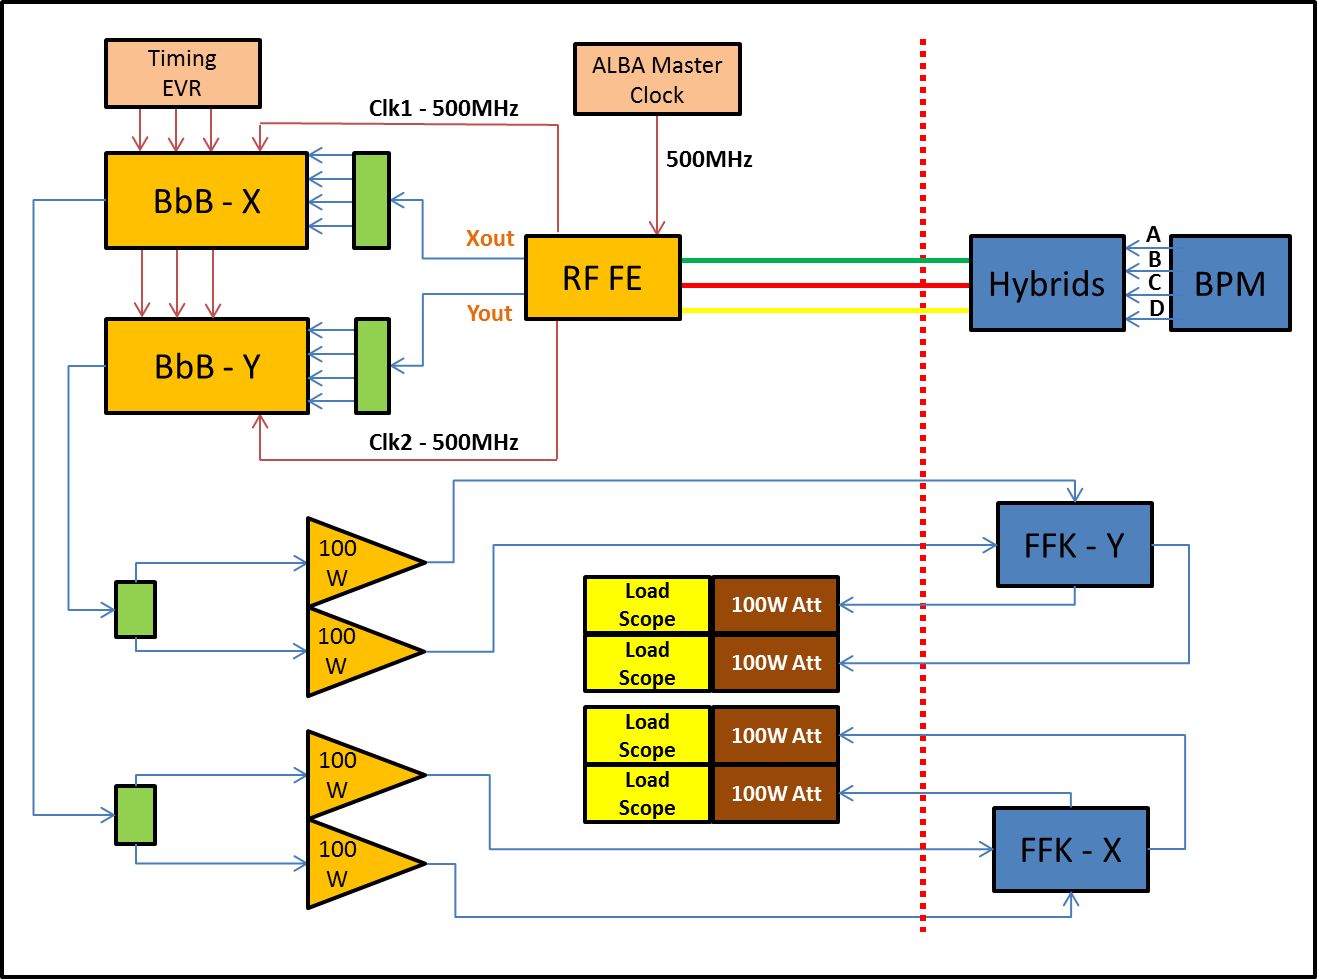
\includegraphics[width=76mm]{img/TUPB046f1}
   \caption{Schematic of the TMBF.}
   \label{layout}
\end{figure}

\begin{figure}[hbt!]
   \centering
   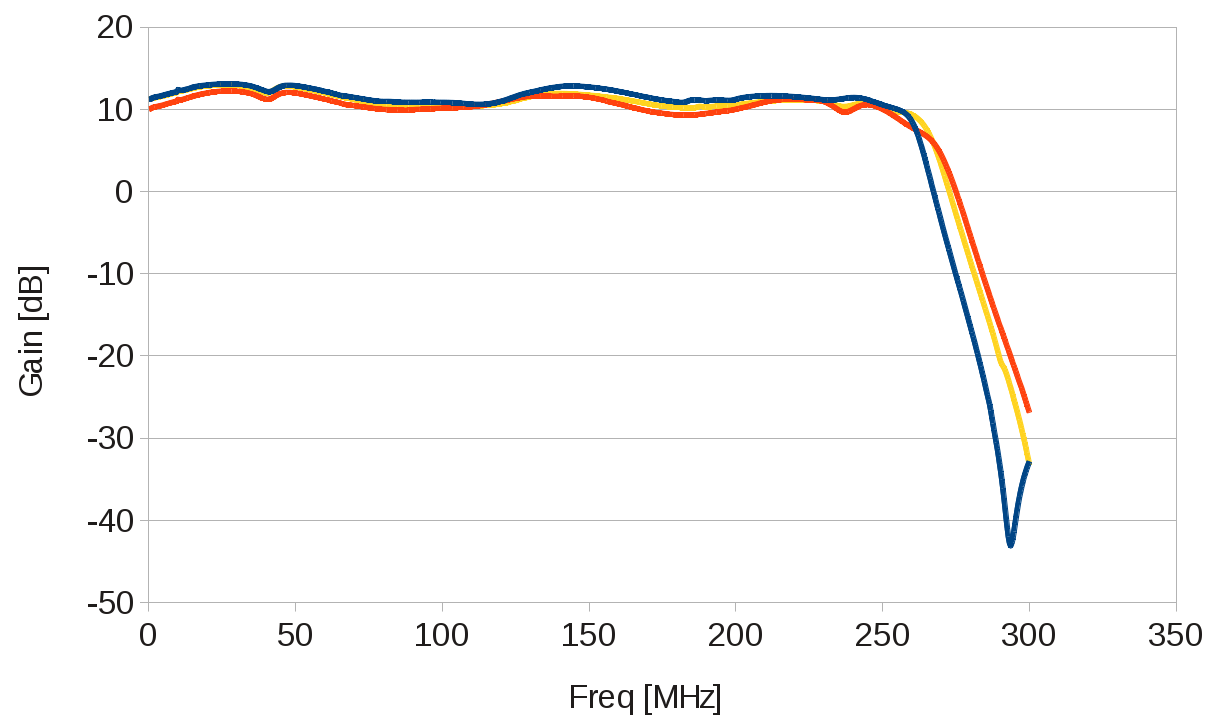
\includegraphics[width=76mm]{img/TUPB046f2}
   \caption{Gain response of three IFI amplifiers. Measurement was done using a 40dB attenuator, so the actual amplifiers gain was around the specified 50dB.}
   \label{AMPLI:GAIN}
\end{figure}

\begin{figure}[hbt!]
   \centering
   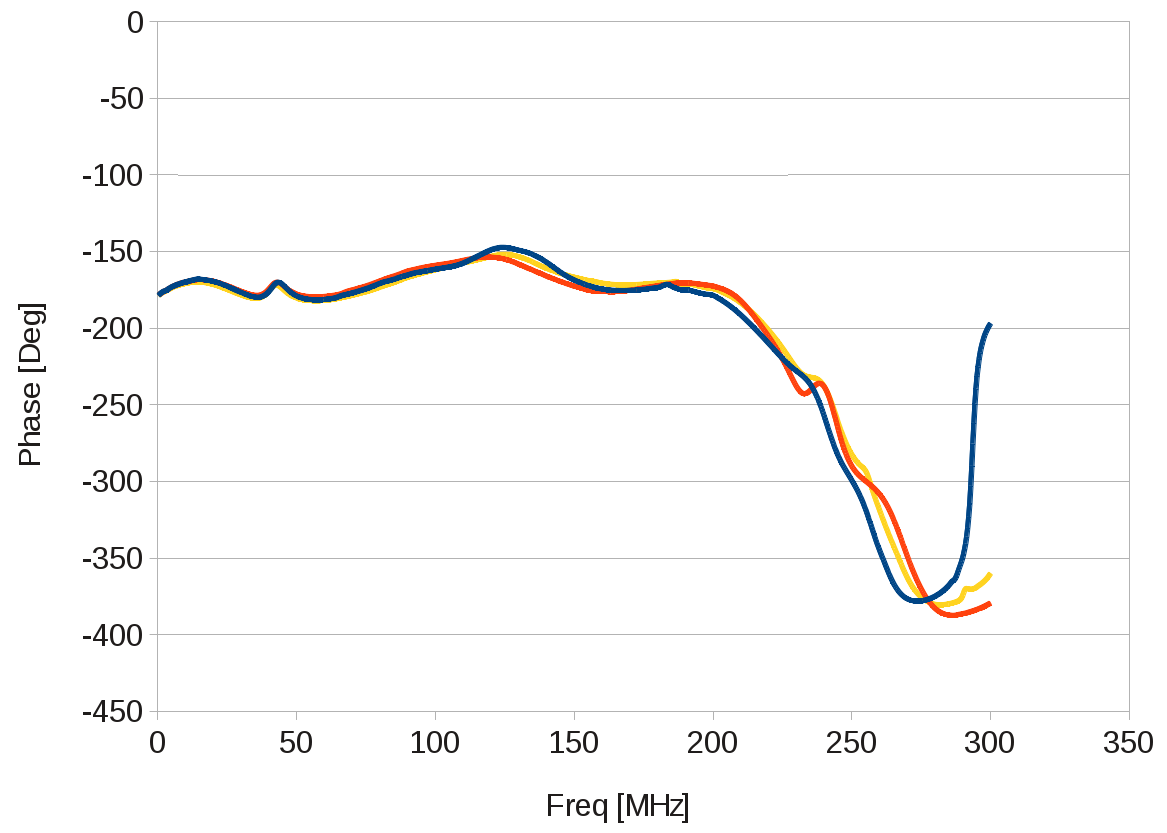
\includegraphics[width=76mm]{img/TUPB046f3}
   \caption{Phase response of three IFI amplifiers. Clear degradation is observed from 200MHz on.}
   \label{AMPLI:PHASE}
\end{figure}


\section{Control Software}

DLS developed its own FPGA implementation to be run in the Libera Bunch-by-Bunch, replacing the one provided by factory. DLS also developed an EPICS driver for controlling 
the system, including an EPICS IOC meant to be run inside the unit, a user interface based on Extensible Display Manager (EDM) together with python and Matlab scripts and some other software utilities~\cite{DLS:IBIC15, DLS:EPAC08, DLS:IBIC13}. 
Since ALBA uses Tango as machine control system, we installed EPICS Base on some selected machines for running the user EDM. Great effort has been done by DLS to prepare a working software infrastructure to adapt all EPICS developments to the ALBA environment, including also the migration of the whole FPGA code from System Verilog to VHDL languages. Next steps regarding the interfacing of the TMBF will be the integration of the EPICS controls into the ALBA Tango system by the use of the so-called \textit{cothread} binding~\cite{DLS:cothread}.

In addition to the instabilities damping capabilities, which is the main application of the system, the control software includes several features for machine studies~\cite{DLS:IBIC15}: 
\begin{itemize}
\item Frequency response compensation using and input (ADC) and output (DAC) gain pre-emphasis with a 3 point FIR.
\item Program sequencing: This allows to apply different control parameters at the same time as data acquisition.
\item Tune detection and fast tune tracking via Phase Locked Loop (PLL) excitation of either one or many bunches.
\item Concurrent sweep tune measurements on up to four bunches. 
\item Separate feedback parameters for individual bunches (useful for hybrid filling patterns). 
\end{itemize}

\section{TMBF Commissioning}

Due to some problems in the power amplifiers, for the time being we have only commissioned the TMBF in the vertical plane. 
For a proper TMBF performance, the phase/delay match throughout the different TMBF components and cables must be carefully checked. This is particularly sensitive in the Hybrid combiner, because phase match tolerances at 1.5~GHz are quite stringent: for a 10$^{\circ}$ tolerance, this is equivalent to cable lengths in the order of 10~mm. 

Figure~\ref{pulse:synchro} shows both the input pulse and the beam passage as seen by one of the electrodes in the vertical kicker. In order to synchronize the bunch passage with the TMBF pulse, we added a 1~ns length cable upstream the amplifier input. Other cable studies to optimize the TMBF performance are shown in Ref.~\cite{MA:cables}.

\begin{figure}[hbt!]
   \centering
   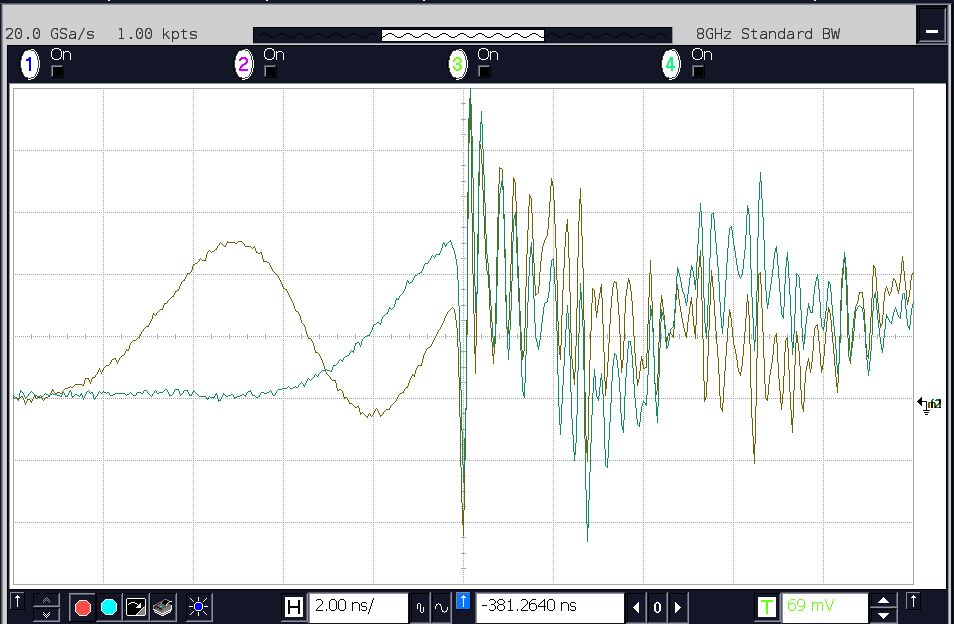
\includegraphics[width=76mm]{img/TUPB046f4}
   \caption{TMBF pulse and bunch passage (high frequency signal at t=0) for the original case (brown trace) and after adding 1~ns length cable (blue trace). Other 4~ns shift (i.e., two buckets) is done using the TMBF GUI. }
   \label{pulse:synchro}
\end{figure}

\subsection{Closing the Loop}

Configuration of the different subsystems to close the feedback loop started with the proper gain and phase setting of the RF FrontEnd to have the highest components levels at Libera Bunch-by-Bunch inputs. Then, in order to enhance the possible beam instabilities, we decreased the vertical chromaticity of the uniform filled beam (440 buckets out of 448) to almost 0. As expected, the vertical instability started at around 40~mA due to Resistive Wall (RW), consistent with studies at~\cite{Thomas}. At this point, the injection was halted to find the proper feedback phase that closes the loop, which could be seen by a reduction in the beam size. Finally, we adjusted the loop gain, the injection was resumed and we could inject up to 110~mA keeping the beam instabilities under control (see Fig.~\ref{DCCT:sigmas}). 

\begin{figure}[hbt!]
   \centering
   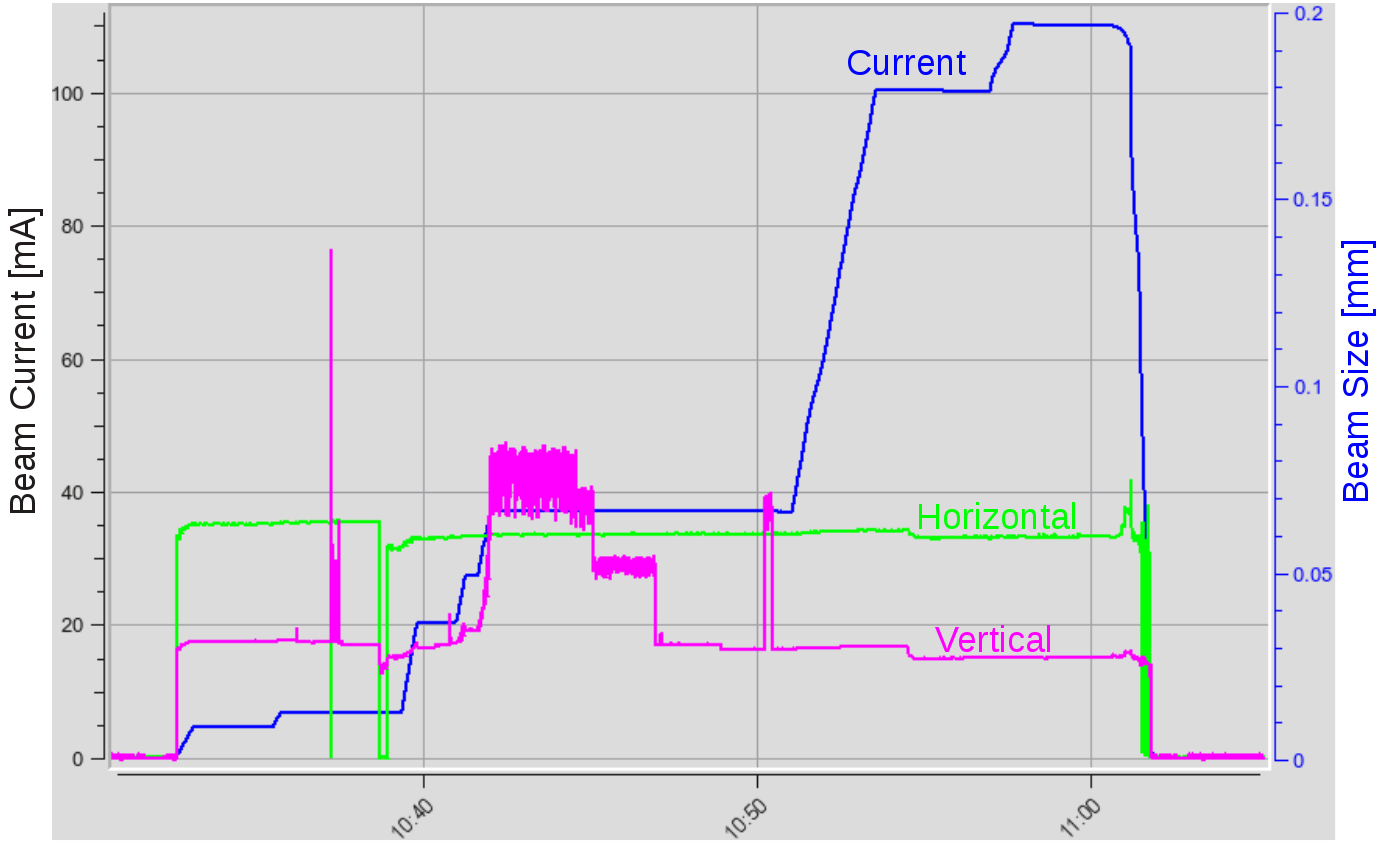
\includegraphics[width=76mm]{img/TUPB046f5}
   \caption{Injection up to 110~mA with vertical $\xi_V \approx 0$. The beam becomes unstable when reaching 40mA and the vertical beam size (pink trace) increases from 28 to 70~$\mu$m. Instabilities are next damped by switching the TMBF ON.}
   \label{DCCT:sigmas}
\end{figure}

\section{TMBF Performance}

Figure~\ref{pinhole:pic} shows a pinhole image with the TMBF OFF, at an intermediate gain of -42~dB, and after fully correction at 0~dB. Currently, with TMBF OFF, to avoid beam instabilities we are obliged to operate the machine at vertical chromaticity $\xi_V\sim$3.5, and use an odd filling pattern in which we fill the machine with 10 trains of 32 bunches each spaced by gaps of 24~ns (in total, 320bunches). 

With the TMBF ON, we can fill the machine with $\xi_V \sim 0$ and use an almost uniform filling pattern, increasing the number of bunches from 320 until 440. Thus, the ALBA performance is improved because the injection efficiency improves and the lifetime increases by about 25\%.  
So far, the TMBF has been left running for 8~h tests without problems during machine shifts, and it is expected to start operating in users mode in September 2015. Meanwhile, other machine tests have been also carried out. 

\begin{figure}[hbt!]
   \centering
   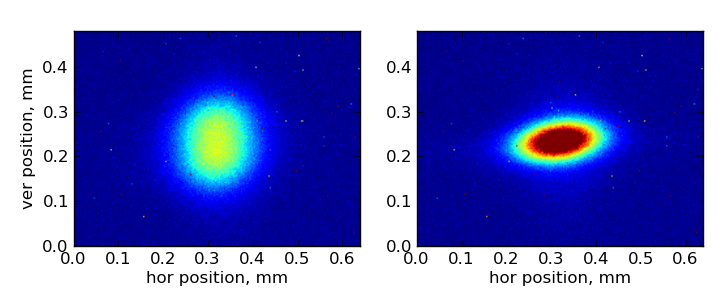
\includegraphics[width=76mm]{img/TUPB046f6}   
   \caption{Beam image with TMBF Off (left) and On (right).}
   \label{pinhole:pic}
\end{figure}

\subsection{Mode Damping Scan}

One of the TMBF features allows to program sequences that apply different control parameters at the same time as data acquisition. This is used to measure the growth rates of the individual multi-bunch modes, and to assess the most dangerous modes for ALBA. 

We program a "super-sequence" that starts from an unstable beam, which is stabilized with the TMBF. We then excite mode "m" using a Numerically Controlled Oscillator (NCO), and we measure its growth time. We then switch it back On and measure its damping time as well. The sequence is then repeated for mode "m+1" and a full characterization spans up to mode 448. The "super-sequence" is also repeated with the TMBF Off (unstable beam) and the results are shown in Fig.~\ref{damping:modes}, where one can see (blue trace) that the most unstable modes (with positive growth rates) are modes between [440,..., 447] (or equivalent, [-1, ... -7]), which indicates the presence of RW instabilities. On the other hand, there also exists mode 324 (or m=-124), which needs further investigations. In any case, all modes are efficiently damped with the TMBF On (at least for these beam settings, 100~mA and $\xi_V \sim 0$).  

\begin{figure}[hbt!]
   \centering
   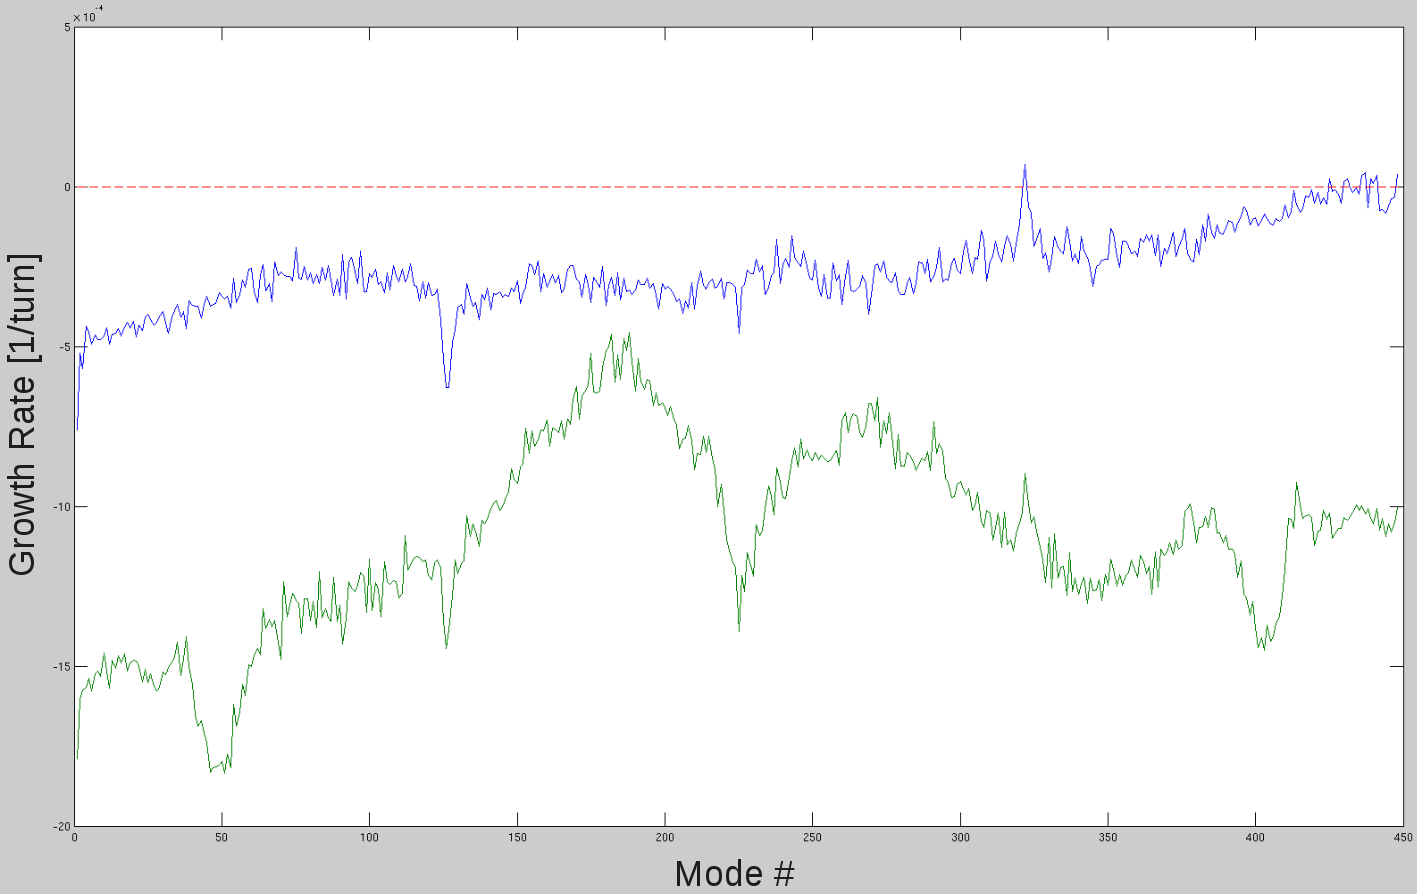
\includegraphics[width=78mm]{img/TUPB046f7}
   \caption{Growth rate for the 448 modes with TMBF On (green) and Off (blue) for a beam of 100~mA and $\xi_V\sim 0$.}
   \label{damping:modes}
\end{figure}

\subsection{Tune Measurements}

Tune measurements can be done in two ways with the TMBF: using the classical method of sweep excitation and detection of one (or many) bunches, or using a tune tracking employing a PLL. This method excites one (or many) bunches using the NCO, detects the phase of the bunches relative to the excitation, and feeds it back through a proportional-integral controller to the NCO frequency. This allows to measure the tune with a precision that can go down to $10^{-5}$. 

\begin{figure}[hbt!]
   \centering
   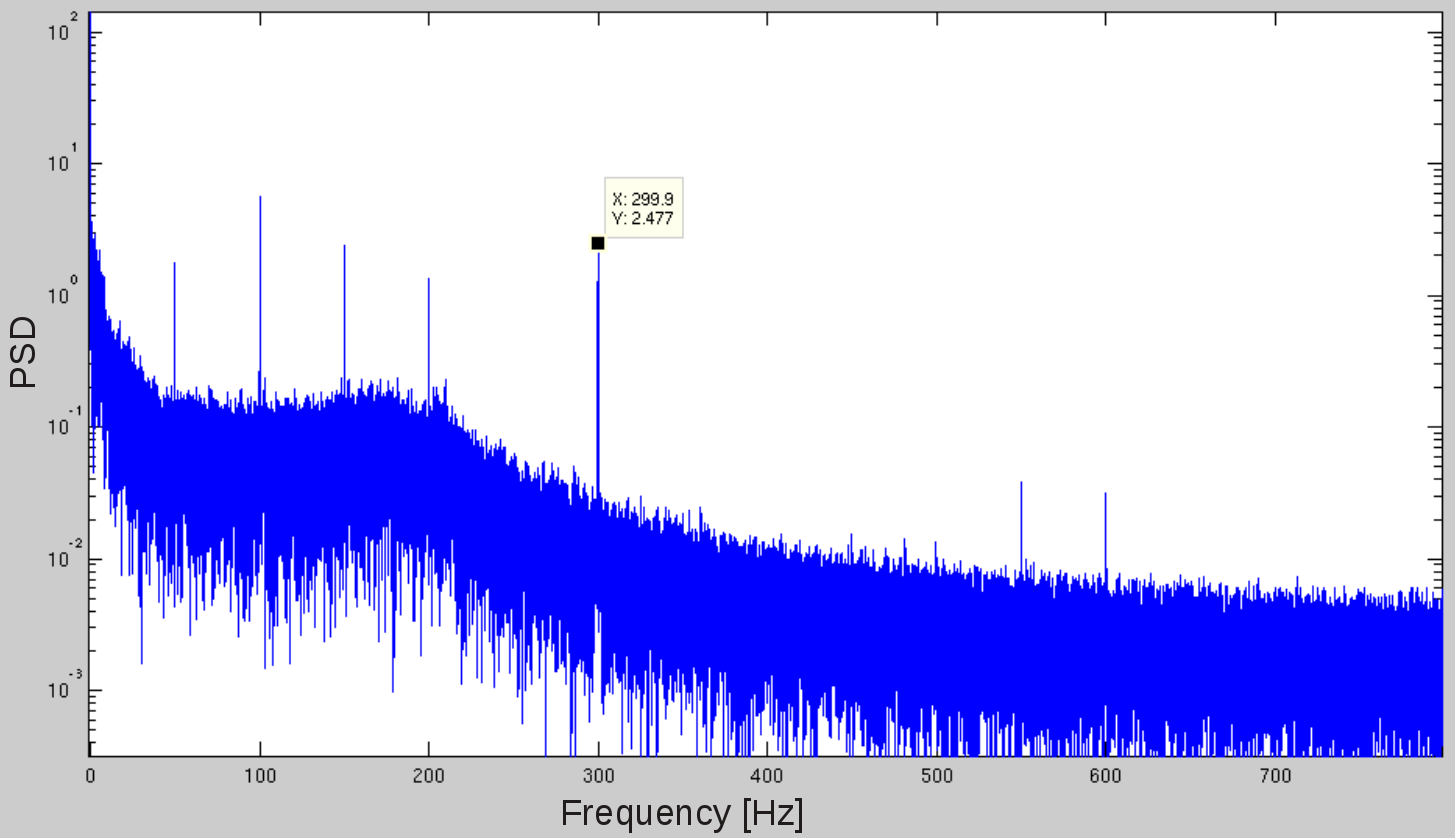
\includegraphics[width=76mm]{img/TUPB046f8}
   \caption{Tune Jitter measured with the fast tune tracking.}
   \label{tune:jitter}
\end{figure}

The tune measurement rate depends on the number of turns to detect the beam phase, which is configurable and typically last for 100 or 200 turns. The buffer that stores this tune measurement can be up to 4096 samples, but it can be read out every time it is updated. Using this capability, the TMBF allows to monitor the tune in long terms and thus monitor, for example, the tune jitter with high precision: Figure~\ref{tune:jitter} shows the spectral density obtained after monitoring the vertical betatron tune during 70~s every 200~turns. One can see that most of the tune jitter is at low frequencies (below 10~Hz), but there also exists peaks at 50~Hz and its harmonics (particularly, the 300~Hz corresponding the power supplies). 


\begin{figure}[t]
   \centering
   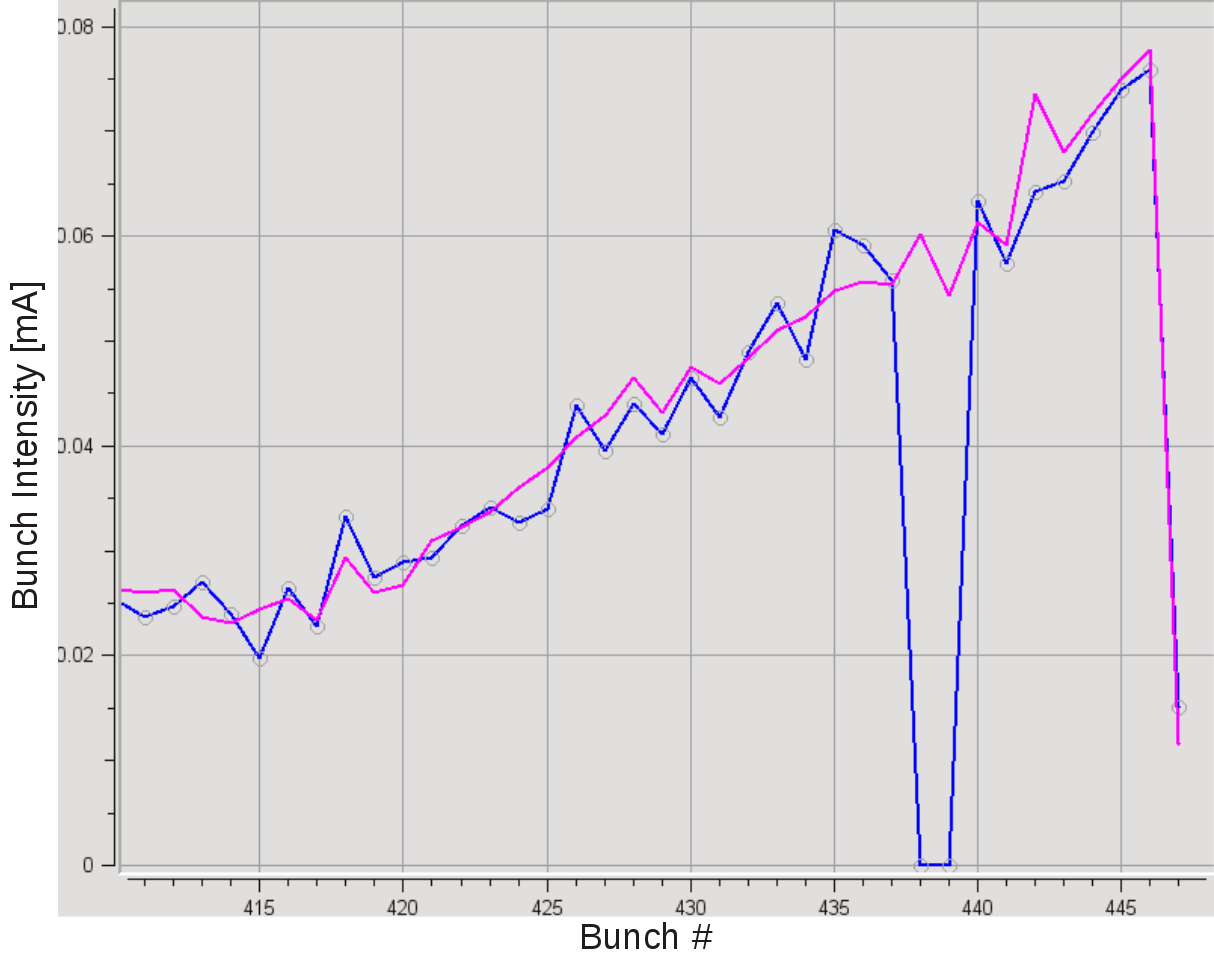
\includegraphics[width=78mm]{img/TUPB046f9}
   \caption{Bunch intensity for buckets between 410 and 448 before (pink trace) and after bunch cleaning (blue trace). }
   \label{bcleaning:MBM}
\end{figure}

\begin{figure}[t]
   \centering
   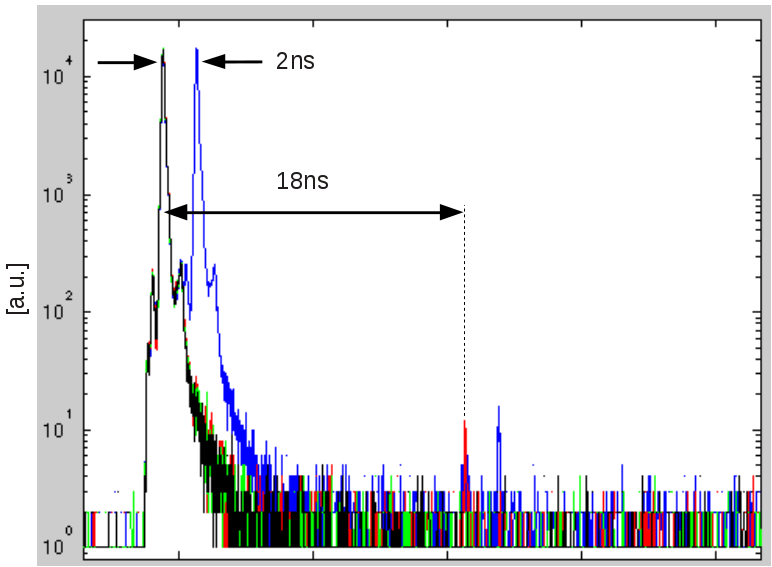
\includegraphics[width=76mm]{img/TUPB046f10}
   \caption{Bunch intensity (in arbitrary units) as measured with the photon counting. Initially, the machine was filled with two consecutive bunches (blue trace), and we noted that two more bunches were filled 18~ns later. We then proceed to kill the different bunches one by one (red and green traces), until we left the machine with only one bunch (black trace).   }
   \label{bcleaning:SBM}
\end{figure}

\subsection{Bunch Cleaning}


Bunch cleaning is performed by exciting the target bunch with a backwards frequency sweep around the vertical betatron tune, and slightly closing the vertical scraper from the nominal position (9.5~mm gap) to 7~mm. 

A first attempt to kill one bunch is shown in Fig.~\ref{bcleaning:MBM}, where the target bunch was initially bunch 438. However, by comparing the traces before (pink) and after (blue), actually two bunches were killed. This is a consequence of the bad phase response of the amplifiers (see Fig.~\ref{AMPLI:PHASE}), which spreads the single kick produced by the Libera Bunch-by-Bunch to actually two bunches.  



Nevertheless, we could see by filling the ring with two consecutive bunches, that optimum settings can be achieved to kill the second bunch (see Fig.~\ref{bcleaning:SBM}). Moreover, this experiment allowed us to realize that our Linac produces a parasitic bunch after 18~ns from the target buckets whose purity is about $10^{-3}$ (from reasons yet to be understood). However, by using the TMBF, we were able to clean also these parasitic bunches and finally leave the machine with a pure single bunch (black trace). 


\section{Summary}
\balance
The implementation of the DLS TMBF system at ALBA has been demonstrated, both in terms of software integration and feedback capabilities. Moreover, extra features have been also tested and proved to be excellent tools for machine studies. In the future, we plan to slightly change our TMBF schematic to add high power splitters after the amplifiers so only one amplifier per plane will be needed. The commissioning of the Horizontal plane and the final integration of the TMBF into the ALBA Tango control system are also to be done now that we have proved that the system behaves as expected.

\section{Acknowledgments}

We would like to acknowledge M. Álvarez for his technical support on the RF measurements of the different system devices.


\iffalse  % only for "biblatex"
	\newpage
	\printbibliography

% "biblatex" is not used, go the "manual" way
\else

%\begin{thebibliography}{9}   % Use for  1-9  references
\begin{thebibliography}{9} % Use for 10-99 references

\bibitem{iTech}
Libera Bunch-by-Bunch, Instrumentation Technologies. http://www.i-tech.si

\bibitem{DLS:IBIC15}
G.~Rehm, M.G.~Abbott, A.F.~Morgan, {\it New features and measurements using the upgraded TMBF at Diamond}, Proc. of IBIC'14, Monterey (USA). 

\bibitem{DLS:EPAC08}
A.F.~Morgan, G.~Rehm, I. Uzun, {\it Performance and features of the Diamond TMBF system}, Proc. of EPAC08, Genoa (Italy). 

\bibitem{DLS:IBIC13}
M.G.~Abbott, G.~Rehm, I.S.~Uzun, {\it Capability Upgrade of the Diamond Transverse Multibunch Feedback}, Proc. of IBIC13, Oxford (UK). 

\bibitem{DLS:cothread}
http://controls.diamond.ac.uk/downloads/python/cothread/

\bibitem{MA:cables}
M.~Alvarez and U.~Iriso, {\it SR FFK CABLES STUDY}, ALBA Internal Report AAD-SRDIFFK-TR-0002 (2012).

\bibitem{Thomas}
T.~Guenzel, {\it Impedance and instabilities for ALBA}, Proc. of EPAC08, Genova (Italy). 

\end{thebibliography}
\vspace{0mm}
\fi

\end{document}